%%%%%%%%%%%%%%%%%%%%%%%%%%%%%% -*- Mode: Latex -*- %%%%%%%%%%%%%%%%%%%%%%%%%%%%
%% 04-11.tex -- IEEE Software Paper on Telemetry
%% Author          : Philip Johnson
%% Created On      : Mon Sep 23 11:52:28 2002
%% Last Modified By: Philip M. Johnson
%% Last Modified On: Thu Jan 20 10:01:44 2005
%% RCS: $Id$
%%%%%%%%%%%%%%%%%%%%%%%%%%%%%%%%%%%%%%%%%%%%%%%%%%%%%%%%%%%%%%%%%%%%%%%%%%%%%%%
%%   Copyright (C) 2002 Philip Johnson
%%%%%%%%%%%%%%%%%%%%%%%%%%%%%%%%%%%%%%%%%%%%%%%%%%%%%%%%%%%%%%%%%%%%%%%%%%%%%%%
%% 

%% Review: David Zubrow/SEI

\documentclass[11pt,twocolumn]{article} 
% Psfig/TeX 
\def\PsfigVersion{1.9}
% dvips version
%
% All psfig/tex software, documentation, and related files
% in this distribution of psfig/tex are 
% Copyright 1987, 1988, 1991 Trevor J. Darrell
%
% Permission is granted for use and non-profit distribution of psfig/tex 
% providing that this notice is clearly maintained. The right to
% distribute any portion of psfig/tex for profit or as part of any commercial
% product is specifically reserved for the author(s) of that portion.
%
% *** Feel free to make local modifications of psfig as you wish,
% *** but DO NOT post any changed or modified versions of ``psfig''
% *** directly to the net. Send them to me and I'll try to incorporate
% *** them into future versions. If you want to take the psfig code 
% *** and make a new program (subject to the copyright above), distribute it, 
% *** (and maintain it) that's fine, just don't call it psfig.
%
% Bugs and improvements to trevor@media.mit.edu.
%
% Thanks to Greg Hager (GDH) and Ned Batchelder for their contributions
% to the original version of this project.
%
% Modified by J. Daniel Smith on 9 October 1990 to accept the
% %%BoundingBox: comment with or without a space after the colon.  Stole
% file reading code from Tom Rokicki's EPSF.TEX file (see below).
%
% More modifications by J. Daniel Smith on 29 March 1991 to allow the
% the included PostScript figure to be rotated.  The amount of
% rotation is specified by the "angle=" parameter of the \psfig command.
%
% Modified by Robert Russell on June 25, 1991 to allow users to specify
% .ps filenames which don't yet exist, provided they explicitly provide
% boundingbox information via the \psfig command. Note: This will only work
% if the "file=" parameter follows all four "bb???=" parameters in the
% command. This is due to the order in which psfig interprets these params.
%
%  3 Jul 1991	JDS	check if file already read in once
%  4 Sep 1991	JDS	fixed incorrect computation of rotated
%			bounding box
% 25 Sep 1991	GVR	expanded synopsis of \psfig
% 14 Oct 1991	JDS	\fbox code from LaTeX so \psdraft works with TeX
%			changed \typeout to \ps@typeout
% 17 Oct 1991	JDS	added \psscalefirst and \psrotatefirst
%

% From: gvr@cs.brown.edu (George V. Reilly)
%
% \psdraft	draws an outline box, but doesn't include the figure
%		in the DVI file.  Useful for previewing.
%
% \psfull	includes the figure in the DVI file (default).
%
% \psscalefirst width= or height= specifies the size of the figure
% 		before rotation.
% \psrotatefirst (default) width= or height= specifies the size of the
% 		 figure after rotation.  Asymetric figures will
% 		 appear to shrink.
%
% \psfigurepath#1	sets the path to search for the figure
%
% \psfig
% usage: \psfig{file=, figure=, height=, width=,
%			bbllx=, bblly=, bburx=, bbury=,
%			rheight=, rwidth=, clip=, angle=, silent=}
%
%	"file" is the filename.  If no path name is specified and the
%		file is not found in the current directory,
%		it will be looked for in directory \psfigurepath.
%	"figure" is a synonym for "file".
%	By default, the width and height of the figure are taken from
%		the BoundingBox of the figure.
%	If "width" is specified, the figure is scaled so that it has
%		the specified width.  Its height changes proportionately.
%	If "height" is specified, the figure is scaled so that it has
%		the specified height.  Its width changes proportionately.
%	If both "width" and "height" are specified, the figure is scaled
%		anamorphically.
%	"bbllx", "bblly", "bburx", and "bbury" control the PostScript
%		BoundingBox.  If these four values are specified
%               *before* the "file" option, the PSFIG will not try to
%               open the PostScript file.
%	"rheight" and "rwidth" are the reserved height and width
%		of the figure, i.e., how big TeX actually thinks
%		the figure is.  They default to "width" and "height".
%	The "clip" option ensures that no portion of the figure will
%		appear outside its BoundingBox.  "clip=" is a switch and
%		takes no value, but the `=' must be present.
%	The "angle" option specifies the angle of rotation (degrees, ccw).
%	The "silent" option makes \psfig work silently.
%

% check to see if macros already loaded in (maybe some other file says
% "\input psfig") ...
\ifx\undefined\psfig\else\endinput\fi

%
% from a suggestion by eijkhout@csrd.uiuc.edu to allow
% loading as a style file. Changed to avoid problems
% with amstex per suggestion by jbence@math.ucla.edu

\let\LaTeXAtSign=\@
\let\@=\relax
\edef\psfigRestoreAt{\catcode`\@=\number\catcode`@\relax}
%\edef\psfigRestoreAt{\catcode`@=\number\catcode`@\relax}
\catcode`\@=11\relax
\newwrite\@unused
\def\ps@typeout#1{{\let\protect\string\immediate\write\@unused{#1}}}
\ps@typeout{psfig/tex \PsfigVersion}

%% Here's how you define your figure path.  Should be set up with null
%% default and a user useable definition.

\def\figurepath{./}
\def\psfigurepath#1{\edef\figurepath{#1}}

%
% @psdo control structure -- similar to Latex @for.
% I redefined these with different names so that psfig can
% be used with TeX as well as LaTeX, and so that it will not 
% be vunerable to future changes in LaTeX's internal
% control structure,
%
\def\@nnil{\@nil}
\def\@empty{}
\def\@psdonoop#1\@@#2#3{}
\def\@psdo#1:=#2\do#3{\edef\@psdotmp{#2}\ifx\@psdotmp\@empty \else
    \expandafter\@psdoloop#2,\@nil,\@nil\@@#1{#3}\fi}
\def\@psdoloop#1,#2,#3\@@#4#5{\def#4{#1}\ifx #4\@nnil \else
       #5\def#4{#2}\ifx #4\@nnil \else#5\@ipsdoloop #3\@@#4{#5}\fi\fi}
\def\@ipsdoloop#1,#2\@@#3#4{\def#3{#1}\ifx #3\@nnil 
       \let\@nextwhile=\@psdonoop \else
      #4\relax\let\@nextwhile=\@ipsdoloop\fi\@nextwhile#2\@@#3{#4}}
\def\@tpsdo#1:=#2\do#3{\xdef\@psdotmp{#2}\ifx\@psdotmp\@empty \else
    \@tpsdoloop#2\@nil\@nil\@@#1{#3}\fi}
\def\@tpsdoloop#1#2\@@#3#4{\def#3{#1}\ifx #3\@nnil 
       \let\@nextwhile=\@psdonoop \else
      #4\relax\let\@nextwhile=\@tpsdoloop\fi\@nextwhile#2\@@#3{#4}}
% 
% \fbox is defined in latex.tex; so if \fbox is undefined, assume that
% we are not in LaTeX.
% Perhaps this could be done better???
\ifx\undefined\fbox
% \fbox code from modified slightly from LaTeX
\newdimen\fboxrule
\newdimen\fboxsep
\newdimen\ps@tempdima
\newbox\ps@tempboxa
\fboxsep = 3pt
\fboxrule = .4pt
\long\def\fbox#1{\leavevmode\setbox\ps@tempboxa\hbox{#1}\ps@tempdima\fboxrule
    \advance\ps@tempdima \fboxsep \advance\ps@tempdima \dp\ps@tempboxa
   \hbox{\lower \ps@tempdima\hbox
  {\vbox{\hrule height \fboxrule
          \hbox{\vrule width \fboxrule \hskip\fboxsep
          \vbox{\vskip\fboxsep \box\ps@tempboxa\vskip\fboxsep}\hskip 
                 \fboxsep\vrule width \fboxrule}
                 \hrule height \fboxrule}}}}
\fi
%
%%%%%%%%%%%%%%%%%%%%%%%%%%%%%%%%%%%%%%%%%%%%%%%%%%%%%%%%%%%%%%%%%%%
% file reading stuff from epsf.tex
%   EPSF.TEX macro file:
%   Written by Tomas Rokicki of Radical Eye Software, 29 Mar 1989.
%   Revised by Don Knuth, 3 Jan 1990.
%   Revised by Tomas Rokicki to accept bounding boxes with no
%      space after the colon, 18 Jul 1990.
%   Portions modified/removed for use in PSFIG package by
%      J. Daniel Smith, 9 October 1990.
%
\newread\ps@stream
\newif\ifnot@eof       % continue looking for the bounding box?
\newif\if@noisy        % report what you're making?
\newif\if@atend        % %%BoundingBox: has (at end) specification
\newif\if@psfile       % does this look like a PostScript file?
%
% PostScript files should start with `%!'
%
{\catcode`\%=12\global\gdef\epsf@start{%!}}
\def\epsf@PS{PS}
%
\def\epsf@getbb#1{%
%
%   The first thing we need to do is to open the
%   PostScript file, if possible.
%
\openin\ps@stream=#1
\ifeof\ps@stream\ps@typeout{Error, File #1 not found}\else
%
%   Okay, we got it. Now we'll scan lines until we find one that doesn't
%   start with %. We're looking for the bounding box comment.
%
   {\not@eoftrue \chardef\other=12
    \def\do##1{\catcode`##1=\other}\dospecials \catcode`\ =10
    \loop
       \if@psfile
	  \read\ps@stream to \epsf@fileline
       \else{
	  \obeyspaces
          \read\ps@stream to \epsf@tmp\global\let\epsf@fileline\epsf@tmp}
       \fi
       \ifeof\ps@stream\not@eoffalse\else
%
%   Check the first line for `%!'.  Issue a warning message if its not
%   there, since the file might not be a PostScript file.
%
       \if@psfile\else
       \expandafter\epsf@test\epsf@fileline:. \\%
       \fi
%
%   We check to see if the first character is a % sign;
%   if so, we look further and stop only if the line begins with
%   `%%BoundingBox:' and the `(atend)' specification was not found.
%   That is, the only way to stop is when the end of file is reached,
%   or a `%%BoundingBox: llx lly urx ury' line is found.
%
          \expandafter\epsf@aux\epsf@fileline:. \\%
       \fi
   \ifnot@eof\repeat
   }\closein\ps@stream\fi}%
%
% This tests if the file we are reading looks like a PostScript file.
%
\long\def\epsf@test#1#2#3:#4\\{\def\epsf@testit{#1#2}
			\ifx\epsf@testit\epsf@start\else
\ps@typeout{Warning! File does not start with `\epsf@start'.  It may not be a PostScript file.}
			\fi
			\@psfiletrue} % don't test after 1st line
%
%   We still need to define the tricky \epsf@aux macro. This requires
%   a couple of magic constants for comparison purposes.
%
{\catcode`\%=12\global\let\epsf@percent=%\global\def\epsf@bblit{%BoundingBox}}
%
%
%   So we're ready to check for `%BoundingBox:' and to grab the
%   values if they are found.  We continue searching if `(at end)'
%   was found after the `%BoundingBox:'.
%
\long\def\epsf@aux#1#2:#3\\{\ifx#1\epsf@percent
   \def\epsf@testit{#2}\ifx\epsf@testit\epsf@bblit
	\@atendfalse
        \epsf@atend #3 . \\%
	\if@atend	
	   \if@verbose{
		\ps@typeout{psfig: found `(atend)'; continuing search}
	   }\fi
        \else
        \epsf@grab #3 . . . \\%
        \not@eoffalse
        \global\no@bbfalse
        \fi
   \fi\fi}%
%
%   Here we grab the values and stuff them in the appropriate definitions.
%
\def\epsf@grab #1 #2 #3 #4 #5\\{%
   \global\def\epsf@llx{#1}\ifx\epsf@llx\empty
      \epsf@grab #2 #3 #4 #5 .\\\else
   \global\def\epsf@lly{#2}%
   \global\def\epsf@urx{#3}\global\def\epsf@ury{#4}\fi}%
%
% Determine if the stuff following the %%BoundingBox is `(atend)'
% J. Daniel Smith.  Copied from \epsf@grab above.
%
\def\epsf@atendlit{(atend)} 
\def\epsf@atend #1 #2 #3\\{%
   \def\epsf@tmp{#1}\ifx\epsf@tmp\empty
      \epsf@atend #2 #3 .\\\else
   \ifx\epsf@tmp\epsf@atendlit\@atendtrue\fi\fi}


% End of file reading stuff from epsf.tex
%%%%%%%%%%%%%%%%%%%%%%%%%%%%%%%%%%%%%%%%%%%%%%%%%%%%%%%%%%%%%%%%%%%

%%%%%%%%%%%%%%%%%%%%%%%%%%%%%%%%%%%%%%%%%%%%%%%%%%%%%%%%%%%%%%%%%%%
% trigonometry stuff from "trig.tex"
\chardef\psletter = 11 % won't conflict with \begin{letter} now...
\chardef\other = 12

\newif \ifdebug %%% turn me on to see TeX hard at work ...
\newif\ifc@mpute %%% don't need to compute some values
\c@mputetrue % but assume that we do

\let\then = \relax
\def\r@dian{pt }
\let\r@dians = \r@dian
\let\dimensionless@nit = \r@dian
\let\dimensionless@nits = \dimensionless@nit
\def\internal@nit{sp }
\let\internal@nits = \internal@nit
\newif\ifstillc@nverging
\def \Mess@ge #1{\ifdebug \then \message {#1} \fi}

{ %%% Things that need abnormal catcodes %%%
	\catcode `\@ = \psletter
	\gdef \nodimen {\expandafter \n@dimen \the \dimen}
	\gdef \term #1 #2 #3%
	       {\edef \t@ {\the #1}%%% freeze parameter 1 (count, by value)
		\edef \t@@ {\expandafter \n@dimen \the #2\r@dian}%
				   %%% freeze parameter 2 (dimen, by value)
		\t@rm {\t@} {\t@@} {#3}%
	       }
	\gdef \t@rm #1 #2 #3%
	       {{%
		\count 0 = 0
		\dimen 0 = 1 \dimensionless@nit
		\dimen 2 = #2\relax
		\Mess@ge {Calculating term #1 of \nodimen 2}%
		\loop
		\ifnum	\count 0 < #1
		\then	\advance \count 0 by 1
			\Mess@ge {Iteration \the \count 0 \space}%
			\Multiply \dimen 0 by {\dimen 2}%
			\Mess@ge {After multiplication, term = \nodimen 0}%
			\Divide \dimen 0 by {\count 0}%
			\Mess@ge {After division, term = \nodimen 0}%
		\repeat
		\Mess@ge {Final value for term #1 of 
				\nodimen 2 \space is \nodimen 0}%
		\xdef \Term {#3 = \nodimen 0 \r@dians}%
		\aftergroup \Term
	       }}
	\catcode `\p = \other
	\catcode `\t = \other
	\gdef \n@dimen #1pt{#1} %%% throw away the ``pt''
}

\def \Divide #1by #2{\divide #1 by #2} %%% just a synonym

\def \Multiply #1by #2%%% allows division of a dimen by a dimen
       {{%%% should really freeze parameter 2 (dimen, passed by value)
	\count 0 = #1\relax
	\count 2 = #2\relax
	\count 4 = 65536
	\Mess@ge {Before scaling, count 0 = \the \count 0 \space and
			count 2 = \the \count 2}%
	\ifnum	\count 0 > 32767 %%% do our best to avoid overflow
	\then	\divide \count 0 by 4
		\divide \count 4 by 4
	\else	\ifnum	\count 0 < -32767
		\then	\divide \count 0 by 4
			\divide \count 4 by 4
		\else
		\fi
	\fi
	\ifnum	\count 2 > 32767 %%% while retaining reasonable accuracy
	\then	\divide \count 2 by 4
		\divide \count 4 by 4
	\else	\ifnum	\count 2 < -32767
		\then	\divide \count 2 by 4
			\divide \count 4 by 4
		\else
		\fi
	\fi
	\multiply \count 0 by \count 2
	\divide \count 0 by \count 4
	\xdef \product {#1 = \the \count 0 \internal@nits}%
	\aftergroup \product
       }}

\def\r@duce{\ifdim\dimen0 > 90\r@dian \then   % sin(x+90) = sin(180-x)
		\multiply\dimen0 by -1
		\advance\dimen0 by 180\r@dian
		\r@duce
	    \else \ifdim\dimen0 < -90\r@dian \then  % sin(-x) = sin(360+x)
		\advance\dimen0 by 360\r@dian
		\r@duce
		\fi
	    \fi}

\def\Sine#1%
       {{%
	\dimen 0 = #1 \r@dian
	\r@duce
	\ifdim\dimen0 = -90\r@dian \then
	   \dimen4 = -1\r@dian
	   \c@mputefalse
	\fi
	\ifdim\dimen0 = 90\r@dian \then
	   \dimen4 = 1\r@dian
	   \c@mputefalse
	\fi
	\ifdim\dimen0 = 0\r@dian \then
	   \dimen4 = 0\r@dian
	   \c@mputefalse
	\fi
%
	\ifc@mpute \then
        	% convert degrees to radians
		\divide\dimen0 by 180
		\dimen0=3.141592654\dimen0
%
		\dimen 2 = 3.1415926535897963\r@dian %%% a well-known constant
		\divide\dimen 2 by 2 %%% we only deal with -pi/2 : pi/2
		\Mess@ge {Sin: calculating Sin of \nodimen 0}%
		\count 0 = 1 %%% see power-series expansion for sine
		\dimen 2 = 1 \r@dian %%% ditto
		\dimen 4 = 0 \r@dian %%% ditto
		\loop
			\ifnum	\dimen 2 = 0 %%% then we've done
			\then	\stillc@nvergingfalse 
			\else	\stillc@nvergingtrue
			\fi
			\ifstillc@nverging %%% then calculate next term
			\then	\term {\count 0} {\dimen 0} {\dimen 2}%
				\advance \count 0 by 2
				\count 2 = \count 0
				\divide \count 2 by 2
				\ifodd	\count 2 %%% signs alternate
				\then	\advance \dimen 4 by \dimen 2
				\else	\advance \dimen 4 by -\dimen 2
				\fi
		\repeat
	\fi		
			\xdef \sine {\nodimen 4}%
       }}

% Now the Cosine can be calculated easily by calling \Sine
\def\Cosine#1{\ifx\sine\UnDefined\edef\Savesine{\relax}\else
		             \edef\Savesine{\sine}\fi
	{\dimen0=#1\r@dian\advance\dimen0 by 90\r@dian
	 \Sine{\nodimen 0}
	 \xdef\cosine{\sine}
	 \xdef\sine{\Savesine}}}	      
% end of trig stuff
%%%%%%%%%%%%%%%%%%%%%%%%%%%%%%%%%%%%%%%%%%%%%%%%%%%%%%%%%%%%%%%%%%%%

\def\psdraft{
	\def\@psdraft{0}
	%\ps@typeout{draft level now is \@psdraft \space . }
}
\def\psfull{
	\def\@psdraft{100}
	%\ps@typeout{draft level now is \@psdraft \space . }
}

\psfull

\newif\if@scalefirst
\def\psscalefirst{\@scalefirsttrue}
\def\psrotatefirst{\@scalefirstfalse}
\psrotatefirst

\newif\if@draftbox
\def\psnodraftbox{
	\@draftboxfalse
}
\def\psdraftbox{
	\@draftboxtrue
}
\@draftboxtrue

\newif\if@prologfile
\newif\if@postlogfile
\def\pssilent{
	\@noisyfalse
}
\def\psnoisy{
	\@noisytrue
}
\psnoisy
%%% These are for the option list.
%%% A specification of the form a = b maps to calling \@p@@sa{b}
\newif\if@bbllx
\newif\if@bblly
\newif\if@bburx
\newif\if@bbury
\newif\if@height
\newif\if@width
\newif\if@rheight
\newif\if@rwidth
\newif\if@angle
\newif\if@clip
\newif\if@verbose
\def\@p@@sclip#1{\@cliptrue}


\newif\if@decmpr

%%% GDH 7/26/87 -- changed so that it first looks in the local directory,
%%% then in a specified global directory for the ps file.
%%% RPR 6/25/91 -- changed so that it defaults to user-supplied name if
%%% boundingbox info is specified, assuming graphic will be created by
%%% print time.
%%% TJD 10/19/91 -- added bbfile vs. file distinction, and @decmpr flag

\def\@p@@sfigure#1{\def\@p@sfile{null}\def\@p@sbbfile{null}
	        \openin1=#1.bb
		\ifeof1\closein1
	        	\openin1=\figurepath#1.bb
			\ifeof1\closein1
			        \openin1=#1
				\ifeof1\closein1%
				       \openin1=\figurepath#1
					\ifeof1
					   \ps@typeout{Error, File #1 not found}
						\if@bbllx\if@bblly
				   		\if@bburx\if@bbury
			      				\def\@p@sfile{#1}%
			      				\def\@p@sbbfile{#1}%
							\@decmprfalse
				  	   	\fi\fi\fi\fi
					\else\closein1
				    		\def\@p@sfile{\figurepath#1}%
				    		\def\@p@sbbfile{\figurepath#1}%
						\@decmprfalse
	                       		\fi%
			 	\else\closein1%
					\def\@p@sfile{#1}
					\def\@p@sbbfile{#1}
					\@decmprfalse
			 	\fi
			\else
				\def\@p@sfile{\figurepath#1}
				\def\@p@sbbfile{\figurepath#1.bb}
				\@decmprtrue
			\fi
		\else
			\def\@p@sfile{#1}
			\def\@p@sbbfile{#1.bb}
			\@decmprtrue
		\fi}

\def\@p@@sfile#1{\@p@@sfigure{#1}}

\def\@p@@sbbllx#1{
		%\ps@typeout{bbllx is #1}
		\@bbllxtrue
		\dimen100=#1
		\edef\@p@sbbllx{\number\dimen100}
}
\def\@p@@sbblly#1{
		%\ps@typeout{bblly is #1}
		\@bbllytrue
		\dimen100=#1
		\edef\@p@sbblly{\number\dimen100}
}
\def\@p@@sbburx#1{
		%\ps@typeout{bburx is #1}
		\@bburxtrue
		\dimen100=#1
		\edef\@p@sbburx{\number\dimen100}
}
\def\@p@@sbbury#1{
		%\ps@typeout{bbury is #1}
		\@bburytrue
		\dimen100=#1
		\edef\@p@sbbury{\number\dimen100}
}
\def\@p@@sheight#1{
		\@heighttrue
		\dimen100=#1
   		\edef\@p@sheight{\number\dimen100}
		%\ps@typeout{Height is \@p@sheight}
}
\def\@p@@swidth#1{
		%\ps@typeout{Width is #1}
		\@widthtrue
		\dimen100=#1
		\edef\@p@swidth{\number\dimen100}
}
\def\@p@@srheight#1{
		%\ps@typeout{Reserved height is #1}
		\@rheighttrue
		\dimen100=#1
		\edef\@p@srheight{\number\dimen100}
}
\def\@p@@srwidth#1{
		%\ps@typeout{Reserved width is #1}
		\@rwidthtrue
		\dimen100=#1
		\edef\@p@srwidth{\number\dimen100}
}
\def\@p@@sangle#1{
		%\ps@typeout{Rotation is #1}
		\@angletrue
%		\dimen100=#1
		\edef\@p@sangle{#1} %\number\dimen100}
}
\def\@p@@ssilent#1{ 
		\@verbosefalse
}
\def\@p@@sprolog#1{\@prologfiletrue\def\@prologfileval{#1}}
\def\@p@@spostlog#1{\@postlogfiletrue\def\@postlogfileval{#1}}
\def\@cs@name#1{\csname #1\endcsname}
\def\@setparms#1=#2,{\@cs@name{@p@@s#1}{#2}}
%
% initialize the defaults (size the size of the figure)
%
\def\ps@init@parms{
		\@bbllxfalse \@bbllyfalse
		\@bburxfalse \@bburyfalse
		\@heightfalse \@widthfalse
		\@rheightfalse \@rwidthfalse
		\def\@p@sbbllx{}\def\@p@sbblly{}
		\def\@p@sbburx{}\def\@p@sbbury{}
		\def\@p@sheight{}\def\@p@swidth{}
		\def\@p@srheight{}\def\@p@srwidth{}
		\def\@p@sangle{0}
		\def\@p@sfile{} \def\@p@sbbfile{}
		\def\@p@scost{10}
		\def\@sc{}
		\@prologfilefalse
		\@postlogfilefalse
		\@clipfalse
		\if@noisy
			\@verbosetrue
		\else
			\@verbosefalse
		\fi
}
%
% Go through the options setting things up.
%
\def\parse@ps@parms#1{
	 	\@psdo\@psfiga:=#1\do
		   {\expandafter\@setparms\@psfiga,}}
%
% Compute bb height and width
%
\newif\ifno@bb
\def\bb@missing{
	\if@verbose{
		\ps@typeout{psfig: searching \@p@sbbfile \space  for bounding box}
	}\fi
	\no@bbtrue
	\epsf@getbb{\@p@sbbfile}
        \ifno@bb \else \bb@cull\epsf@llx\epsf@lly\epsf@urx\epsf@ury\fi
}	
\def\bb@cull#1#2#3#4{
	\dimen100=#1 bp\edef\@p@sbbllx{\number\dimen100}
	\dimen100=#2 bp\edef\@p@sbblly{\number\dimen100}
	\dimen100=#3 bp\edef\@p@sbburx{\number\dimen100}
	\dimen100=#4 bp\edef\@p@sbbury{\number\dimen100}
	\no@bbfalse
}
% rotate point (#1,#2) about (0,0).
% The sine and cosine of the angle are already stored in \sine and
% \cosine.  The result is placed in (\p@intvaluex, \p@intvaluey).
\newdimen\p@intvaluex
\newdimen\p@intvaluey
\def\rotate@#1#2{{\dimen0=#1 sp\dimen1=#2 sp
%            	calculate x' = x \cos\theta - y \sin\theta
		  \global\p@intvaluex=\cosine\dimen0
		  \dimen3=\sine\dimen1
		  \global\advance\p@intvaluex by -\dimen3
% 		calculate y' = x \sin\theta + y \cos\theta
		  \global\p@intvaluey=\sine\dimen0
		  \dimen3=\cosine\dimen1
		  \global\advance\p@intvaluey by \dimen3
		  }}
\def\compute@bb{
		\no@bbfalse
		\if@bbllx \else \no@bbtrue \fi
		\if@bblly \else \no@bbtrue \fi
		\if@bburx \else \no@bbtrue \fi
		\if@bbury \else \no@bbtrue \fi
		\ifno@bb \bb@missing \fi
		\ifno@bb \ps@typeout{FATAL ERROR: no bb supplied or found}
			\no-bb-error
		\fi
		%
%\ps@typeout{BB: \@p@sbbllx, \@p@sbblly, \@p@sbburx, \@p@sbbury} 
%
% store height/width of original (unrotated) bounding box
		\count203=\@p@sbburx
		\count204=\@p@sbbury
		\advance\count203 by -\@p@sbbllx
		\advance\count204 by -\@p@sbblly
		\edef\ps@bbw{\number\count203}
		\edef\ps@bbh{\number\count204}
		%\ps@typeout{ psbbh = \ps@bbh, psbbw = \ps@bbw }
		\if@angle 
			\Sine{\@p@sangle}\Cosine{\@p@sangle}
	        	{\dimen100=\maxdimen\xdef\r@p@sbbllx{\number\dimen100}
					    \xdef\r@p@sbblly{\number\dimen100}
			                    \xdef\r@p@sbburx{-\number\dimen100}
					    \xdef\r@p@sbbury{-\number\dimen100}}
%
% Need to rotate all four points and take the X-Y extremes of the new
% points as the new bounding box.
                        \def\minmaxtest{
			   \ifnum\number\p@intvaluex<\r@p@sbbllx
			      \xdef\r@p@sbbllx{\number\p@intvaluex}\fi
			   \ifnum\number\p@intvaluex>\r@p@sbburx
			      \xdef\r@p@sbburx{\number\p@intvaluex}\fi
			   \ifnum\number\p@intvaluey<\r@p@sbblly
			      \xdef\r@p@sbblly{\number\p@intvaluey}\fi
			   \ifnum\number\p@intvaluey>\r@p@sbbury
			      \xdef\r@p@sbbury{\number\p@intvaluey}\fi
			   }
%			lower left
			\rotate@{\@p@sbbllx}{\@p@sbblly}
			\minmaxtest
%			upper left
			\rotate@{\@p@sbbllx}{\@p@sbbury}
			\minmaxtest
%			lower right
			\rotate@{\@p@sbburx}{\@p@sbblly}
			\minmaxtest
%			upper right
			\rotate@{\@p@sbburx}{\@p@sbbury}
			\minmaxtest
			\edef\@p@sbbllx{\r@p@sbbllx}\edef\@p@sbblly{\r@p@sbblly}
			\edef\@p@sbburx{\r@p@sbburx}\edef\@p@sbbury{\r@p@sbbury}
%\ps@typeout{rotated BB: \r@p@sbbllx, \r@p@sbblly, \r@p@sbburx, \r@p@sbbury}
		\fi
		\count203=\@p@sbburx
		\count204=\@p@sbbury
		\advance\count203 by -\@p@sbbllx
		\advance\count204 by -\@p@sbblly
		\edef\@bbw{\number\count203}
		\edef\@bbh{\number\count204}
		%\ps@typeout{ bbh = \@bbh, bbw = \@bbw }
}
%
% \in@hundreds performs #1 * (#2 / #3) correct to the hundreds,
%	then leaves the result in @result
%
\def\in@hundreds#1#2#3{\count240=#2 \count241=#3
		     \count100=\count240	% 100 is first digit #2/#3
		     \divide\count100 by \count241
		     \count101=\count100
		     \multiply\count101 by \count241
		     \advance\count240 by -\count101
		     \multiply\count240 by 10
		     \count101=\count240	%101 is second digit of #2/#3
		     \divide\count101 by \count241
		     \count102=\count101
		     \multiply\count102 by \count241
		     \advance\count240 by -\count102
		     \multiply\count240 by 10
		     \count102=\count240	% 102 is the third digit
		     \divide\count102 by \count241
		     \count200=#1\count205=0
		     \count201=\count200
			\multiply\count201 by \count100
		 	\advance\count205 by \count201
		     \count201=\count200
			\divide\count201 by 10
			\multiply\count201 by \count101
			\advance\count205 by \count201
			%
		     \count201=\count200
			\divide\count201 by 100
			\multiply\count201 by \count102
			\advance\count205 by \count201
			%
		     \edef\@result{\number\count205}
}
\def\compute@wfromh{
		% computing : width = height * (bbw / bbh)
		\in@hundreds{\@p@sheight}{\@bbw}{\@bbh}
		%\ps@typeout{ \@p@sheight * \@bbw / \@bbh, = \@result }
		\edef\@p@swidth{\@result}
		%\ps@typeout{w from h: width is \@p@swidth}
}
\def\compute@hfromw{
		% computing : height = width * (bbh / bbw)
	        \in@hundreds{\@p@swidth}{\@bbh}{\@bbw}
		%\ps@typeout{ \@p@swidth * \@bbh / \@bbw = \@result }
		\edef\@p@sheight{\@result}
		%\ps@typeout{h from w : height is \@p@sheight}
}
\def\compute@handw{
		\if@height 
			\if@width
			\else
				\compute@wfromh
			\fi
		\else 
			\if@width
				\compute@hfromw
			\else
				\edef\@p@sheight{\@bbh}
				\edef\@p@swidth{\@bbw}
			\fi
		\fi
}
\def\compute@resv{
		\if@rheight \else \edef\@p@srheight{\@p@sheight} \fi
		\if@rwidth \else \edef\@p@srwidth{\@p@swidth} \fi
		%\ps@typeout{rheight = \@p@srheight, rwidth = \@p@srwidth}
}
%		
% Compute any missing values
\def\compute@sizes{
	\compute@bb
	\if@scalefirst\if@angle
% at this point the bounding box has been adjsuted correctly for
% rotation.  PSFIG does all of its scaling using \@bbh and \@bbw.  If
% a width= or height= was specified along with \psscalefirst, then the
% width=/height= value needs to be adjusted to match the new (rotated)
% bounding box size (specifed in \@bbw and \@bbh).
%    \ps@bbw       width=
%    -------  =  ---------- 
%    \@bbw       new width=
% so `new width=' = (width= * \@bbw) / \ps@bbw; where \ps@bbw is the
% width of the original (unrotated) bounding box.
	\if@width
	   \in@hundreds{\@p@swidth}{\@bbw}{\ps@bbw}
	   \edef\@p@swidth{\@result}
	\fi
	\if@height
	   \in@hundreds{\@p@sheight}{\@bbh}{\ps@bbh}
	   \edef\@p@sheight{\@result}
	\fi
	\fi\fi
	\compute@handw
	\compute@resv}

%
% \psfig
% usage : \psfig{file=, height=, width=, bbllx=, bblly=, bburx=, bbury=,
%			rheight=, rwidth=, clip=}
%
% "clip=" is a switch and takes no value, but the `=' must be present.
\def\psfig#1{\vbox {
	% do a zero width hard space so that a single
	% \psfig in a centering enviornment will behave nicely
	%{\setbox0=\hbox{\ }\ \hskip-\wd0}
	%
	\ps@init@parms
	\parse@ps@parms{#1}
	\compute@sizes
	%
	\ifnum\@p@scost<\@psdraft{
		%
		\special{ps::[begin] 	\@p@swidth \space \@p@sheight \space
				\@p@sbbllx \space \@p@sbblly \space
				\@p@sbburx \space \@p@sbbury \space
				startTexFig \space }
		\if@angle
			\special {ps:: \@p@sangle \space rotate \space} 
		\fi
		\if@clip{
			\if@verbose{
				\ps@typeout{(clip)}
			}\fi
			\special{ps:: doclip \space }
		}\fi
		\if@prologfile
		    \special{ps: plotfile \@prologfileval \space } \fi
		\if@decmpr{
			\if@verbose{
				\ps@typeout{psfig: including \@p@sfile.Z \space }
			}\fi
			\special{ps: plotfile "`zcat \@p@sfile.Z" \space }
		}\else{
			\if@verbose{
				\ps@typeout{psfig: including \@p@sfile \space }
			}\fi
			\special{ps: plotfile \@p@sfile \space }
		}\fi
		\if@postlogfile
		    \special{ps: plotfile \@postlogfileval \space } \fi
		\special{ps::[end] endTexFig \space }
		% Create the vbox to reserve the space for the figure.
		\vbox to \@p@srheight sp{
		% 1/92 TJD Changed from "true sp" to "sp" for magnification.
			\hbox to \@p@srwidth sp{
				\hss
			}
		\vss
		}
	}\else{
		% draft figure, just reserve the space and print the
		% path name.
		\if@draftbox{		
			% Verbose draft: print file name in box
			\hbox{\frame{\vbox to \@p@srheight sp{
			\vss
			\hbox to \@p@srwidth sp{ \hss \@p@sfile \hss }
			\vss
			}}}
		}\else{
			% Non-verbose draft
			\vbox to \@p@srheight sp{
			\vss
			\hbox to \@p@srwidth sp{\hss}
			\vss
			}
		}\fi	



	}\fi
}}
\psfigRestoreAt
\let\@=\LaTeXAtSign




\usepackage{/export/home/csdl/tex/icse2003/latex8}
\usepackage{times}
%% A verbatim-like environment which allows font changes
%%\usepackage{alltt}
%% New LaTeX2e graphics support
\usepackage[final]{graphicx}
% uncomment the % away on next line to produce the final camera-ready version
% and uncomment the \thispagestyle{empty} following \maketitle
\pagestyle{empty}

\begin{document}

\title{Improving Software Development Management \\ through Software Project Telemetry}


\author{\protect\begin{tabular}{ccc}
Philip M. Johnson & Hongbing Kou & Michael Paulding  \\
Qin Zhang & Aaron Kagawa & Takuya Yamashita \\
\end{tabular}\\
\em  Collaborative Software Development Laboratory \\
\em  Department of Information and Computer Sciences \\
\em  University of Hawai'i \\
\em  Honolulu, HI 96822 \\
\em  johnson@hawaii.edu}
\maketitle
\thispagestyle{empty}

\begin{abstract}  % 200 words

Software project telemetry is a new approach to software project
management in which sensors are attached to development environment tools
to unobtrusively monitor the process and products of development. This
sensor data is abstracted into high-level perspectives on development
trends called Telemetry Reports, which provide project members with 
insights useful for local, in-process decision making.  This paper presents
the essential characteristics of software project telemetry, contrasts it
to other approaches such as predictive models based upon historical
software project data, describes a reference framework implementation of
software project telemetry called Hackystat, and presents our lessons
learned so far. 

\end{abstract}

\Section{Introduction}
\label{sec:intro}

It is conventional wisdom in the software engineering research community
that metrics can improve the effectiveness of project management.
Proponents of software metrics quote theorists and practitioners from
Galileo's ``What is not measurable, make measurable'' \cite{Finkelstein82}
to DeMarco's ``You can neither predict nor control what you cannot
measure'' \cite{DeMarco82}.  Software metrics range from internal product
attributes, such as size, complexity, and modularity, to external process
attributes, such as effort, productivity, testing quality, and reliability
\cite{Fenton97}. 

Despite the potential of metrics in theory, effectively applying them
appears to be far from mainstream in practice. For example, a recent case
study of over 600 software professionals revealed that only 27\% viewed
metrics as ``very'' or ``extremely'' important to their software project
decision making process \cite{Kulik2003}. The study also revealed that cost
and schedule estimation was the only use of metrics attempted
by a majority of respondents.

At least two hypotheses could account for the gulf separating the theory
from the practice of software metrics. The first is that three quarters of
practitioners are just plain uninformed: if they would subscribe to the
journals and/or partake of the many educational opportunities regarding
software metrics, they would immediately implement current ``best
practice'' that would just as quickly improve their project management
decision making.

While all of us, theorists and practitioners alike, can always benefit from
additional reading and education, there is an alternative explanation.
Perhaps the metrics methods used by theorists yield results not easily
translated into practice?  Consider that much metrics research involves the
following basic method: (1) collect a set of process and product
measures (such as size, effort, known defects, complexity, etc.) for a set
of completed software projects; (2) generate a model that fits this data;
(3) claim that this model can now be used to predict characteristics of
future projects. For example, a model might predict that a future project
of size S will require E person-months of effort; another that the future
implementation of a module with complexity C will be prone to defects with
density D. 

Practitioners face several barriers to adoption of these predictive,
model-based approaches to metrics.  First, to use the model unchanged,
practitioners must confirm that the set of projects used to calibrate the
model are similar to their own.  This is the {\em Context Problem}: unless
the context associated with the software process and project data in the
repository is similar to the context associated with the practitioner's
projects, then the applicability of the model's outputs to the practitioner
is in question.  Second, practitioners must also confirm that the context
of their future projects will remain similar to their previous ones.  If
those two conditions cannot be met, then the model cannot be used without
recalibration.  This involves replicating the model-building method
within the practitioner's organization, with the risks that the resulting
model will not work or that the organization may change, rendering the
context of future projects different from those used to calibrate the
model. Third, they must assess the cost associated with metrics collection and analysis, and 
ensure that these costs are balanced by the relevance of the metrics and their interpretation.

Faced with these barriers, it is no wonder that many practitioners find it
daunting to apply metrics best practices to their own situation. Indeed,
the agile community generally argues against model-based metrics
applications, promoting much ``softer'' metrics for decision-making
\cite{Beck00}.

Fortunately, creation of predictive models based upon historical project
data is not the only possible way to apply software metrics to project
management.  In this paper, we present a new approach based upon the notion
of ``telemetry''.

\Section {Software Project Telemetry}

According to Encyclopedia Brittanica, telemetry is a ``highly automated
communications process by which measurements are made and other data
collected at remote or inaccessible points and transmitted to receiving
equipment for monitoring, display, and recording.''  Perhaps the highest
profile user of telemetry is NASA, where telemetry has been used since 1965
to monitor the early Gemini missions to the modern Mars rover flights.  At
NASA's Mission Control Center, for example, dozens of specialists monitor
telemetry data sent from sensors attached to a space vehicle and its
occupants.  This data is used for many purposes, including early warning of
anomalies indicating problems, for better insight into the current status
of the mission, and for the impact of making incremental course or mission
adjustments.

We define ``software project telemetry" as a style of software metrics
definition, collection, and analysis with the following essential
properties:

\begin{enumerate}

\item {\em Software project telemetry data is collected automatically by tools
   that unobtrusively monitor some form of state in the project
   development environment.}  In other words, the software developers are
   working in a ``remote or inaccessable location'' from the perspective of
   metrics collection activities. This contrasts with software metrics data
   that requires human intervention or developer effort to collect, such as
   PSP/TSP metrics \cite{Humphrey95}.
        
\item {\em Software project telemetry data consists of a stream of
   time-stamped events, where the time-stamp is significant for analysis.}
   Software project telemetry data is thus focused on evolutionary
   processes in development.  This contrasts, for example, with Cocomo
   \cite{Boehm81}, where the time at which the calibration data was
   collected about the project is not significant.

\item {\em Software project telemetry data is continuously and immediately 
available to both developers and managers.}  Telemetry data is not hidden
away in some obscure database guarded by the software quality improvement
group.  It is easily visible to all members of the project for 
interpretation. 

\item {\em Software project telemetry exhibits graceful degradation.}
While complete telemetry data provides the best support for project
management, the analyses should not be brittle: they should still provide
value even if complete sensor data is not available. For example, 
telemetry collection and analysis should provide decision-making
value even if these activities start midway through a project.
         
\item {\em Software project telemetry is used for in-process monitoring,
   control, and short-term prediction.} Telemetry analyses provide
   representations of current project state and how it is changing at
   various time scales---we have so far found days, weeks, and months to be
   useful scales.  The simultaneous display of multiple project state values and
   how they change over the same time periods allow opportunistic
   analyses---the emergent knowledge that one state variable appears to
   co-vary with another in the context of the current project.


\end{enumerate}

Software Project Telemetry enables a more incremental, distributed,
visible, and experiential approach to project decision-making. For example,
if one finds that complexity telemetry values are increasing, {\em and}
that defect density telemetry values are also increasing, then one could
try corrective action (such as simplification of overly complex modules)
and see if that results in a decrease in defect density telemetry
values. One can also monitor other telemetry data to see if such
simplification has unintended side-effects (such as performance
degradation).  Project management using telemetry thus involves cycles of
hypothesis generation (Does module complexity correlate with defect
density?), hypothesis testing (If I reduce module complexity, then will
defect density decrease?), and impact analysis (Do the process changes
required to reduce module complexity produce unintended side-effects?).
Finally, Software Project Telemetry supports decentralized project
management: since telemetry data is visible to all members of the project,
it enables all members of the project--developers and managers--to engage
in these management activities.

Software Project Telemetry is related to in-process software metrics, such
as work done on management of software testing \cite{Kan01}. However,
such work tends to focus on a narrow range of measures and management
actions related to testing, and as a result can lead to manual collection and/or analysis of data.  The
broader scope of telemetry necessitates automated collection and analysis,
with a corresponding broader range of management decision-making support.

Software Project Telemetry also relates in interesting ways to both the
Capability Maturity Model Integration (CMMI) and Agile methods. The CMMI is
a revision of the original Capability Maturity Model to incorporate lessons
learned and to support more modern, iterative development processes. In an
article on how to transition from CMM to CMMI, Walker Royce asserts the
importance of ``instrument[ing] the process for objective quality
control. Lifecycle assessments of both the process and all intermediate
products must be tightly integrated into the process, using well-defined
measures derived directly from the evolving engineering artifacts and
integrated into all activities and teams. \cite{Royce02}.''  Software
Project Telemetry appears well suited to the CMMI vision for process
improvement.

Agile method proponents are traditionally suspicious of conventional
process and product measurements and technologies for project decision
making. Jim Highsmith frames the problem as follows: ``Agile approaches
excel in volatile environments in which conformance to plans made months in
advance is a poor measure of success. If agility is important, then one of
the characteristics we should be measuring is that agility. Traditional
measures of success emphasize conformance to predictions (plans). Agility
emphasizes responsiveness to change. So there is a conflict because
managers and executives say that they want flexibility, but then they still
measure success based on conformance to plans. \cite{Highsmith02}.''
Software Project Telemetry provides an infrastructure for measurement that
is not focused on whether a particular long-range target was achieved, but
rather whether the process and product measurements indicate adaptation and
improvement over the recent past. 


\begin{figure*}[ht]
  \centering
  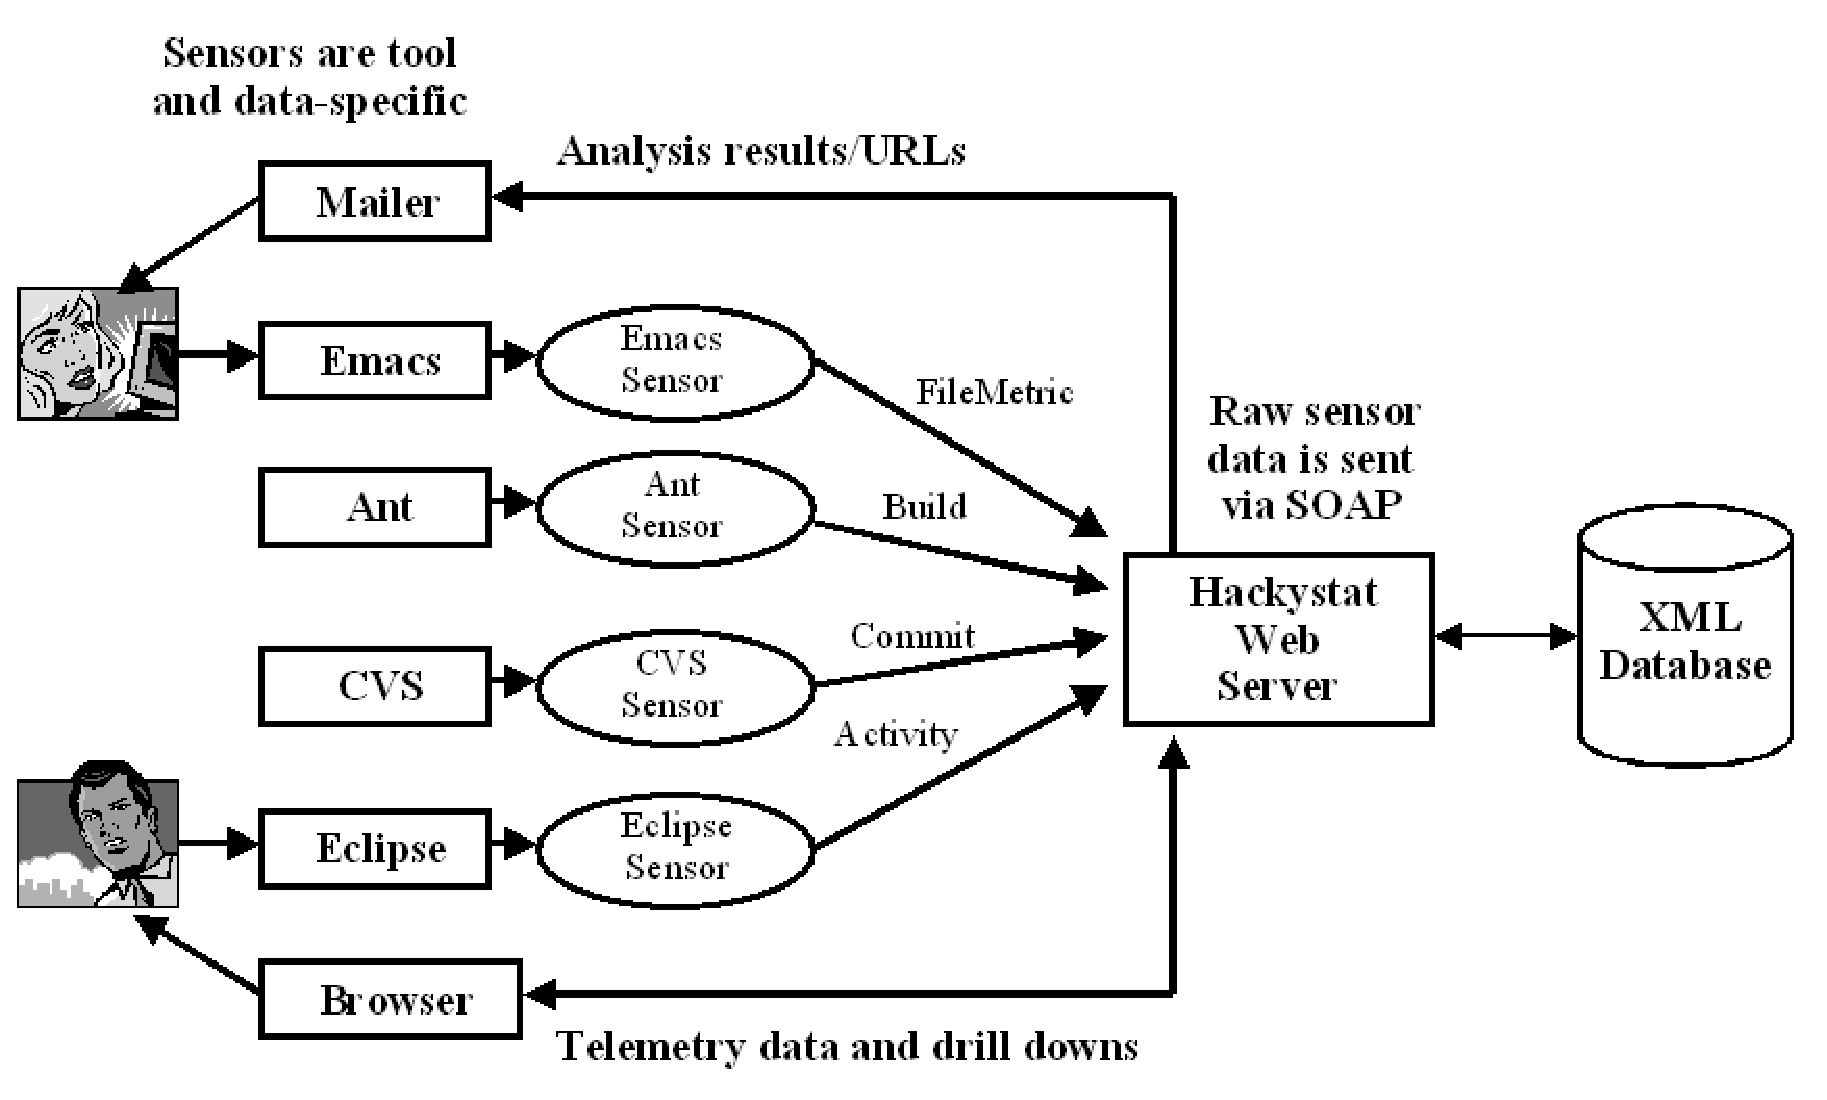
\includegraphics[width=0.75\textwidth]{architecture.eps}
  \caption{The basic architecture of Hackystat. Sensors are attached to
  tools directly invoked by developers (such as Eclipse or Emacs) as
  well as to tools implicitly manipulated by developers (such as CVS or 
  an automated build process using Ant).}
  \label{fig:architecture}
\end{figure*}

\Section{Supporting Software Project Telemetry}

For the past several years, we have been designing, implementing, and
evaluating tools and techniques to support a telemetry-based approach to
software project management as part of Project Hackystat.  Figure
\ref{fig:architecture} illustrates the overall architecture of the
system. First, the project development environment must be instrumented by
installing Hackystat sensors, which developers attach to the various tools
such as their editor, build system, configuration management system, and so
forth. Once installed, the Hackystat sensors unobtrusively monitor
development activities and send process and product data to a centralized
web service.  Project members can log in to the web server to see the
collected raw data and run analyses that integrate and abstract the raw
sensor data streams into telemetry.  Hackystat also allows project members
to configure ``alerts'' that watch for specific conditions in the
telemetry stream and send email when these conditions occur.  

Hackystat supports the following general classes of software project telemetry:

\begin{itemize}

\item {\em Development telemetry} is data gathered by observing the
behavior of project developers and managers as reflected in their tool
usage, and includes information about the files they edit, the time they
spend using various tools, the changes they make to project artifacts, the
sequences of tool or command invocations, and so forth. Development
telemetry can be gathered by attaching sensors to editors, such as Eclipse
or Emacs, to Office applications such as Word or Frontpage, to
configuration management tools such as CVS, to issue management tools such
as Bugzilla or Jira, and so forth.

\item {\em Build telemetry} is data gathered by observing the results of
tools invoked to compile, link, and test the system. Build telemetry can be
gathered from build tools like Ant, Make, or CruiseControl, testing tools
like JUnit, size and complexity tools like LOCC, and so forth.

\item {\em Execution telemetry} is data gathered by observing the behavior of
the system as it executes. This telemetry can be gathered by instrumenting
the run-time environment of the system to collect data about its internal
state (heap size, occurrence of exceptions, etc.) as well as by tools that
perform load or stress testing of the system, such as JMeter.  

\item {\em Usage telemetry} is data gathered by observing the behavior of
users as they interact with the system, such as the frequency, types, and sequences
of command invocations during a given period of time in a given subsystem.

\end{itemize}

For a description of the specific sensors and data types currently supported by
Hackystat, see Section \ref{sec:Sidebar:Sensors}, Sidebar.  


The path from sensors to the telemetry report displayed in Figure
\ref{fig:telemetryreport} involves several steps.  First, ``raw'' sensor
data is collected by observing behavior in various client systems and then
sent to the Hackystat server, which it is persisted in an XML-based
repository.  The raw sensor data is abstracted into ``DailyProjectData''
instances, which can involve the synthesis of sensor data from multiple
group members and/or multiple sensors into a higher level representation of
sensor data for a given project and day.   Sets of DailyProjectData
instances are then manipulated by ``Reduction Functions'', which emit a
sequence of numerical telemetry values for a given project and time scale
of days, weeks, or months.  

The previous steps occur ``below the hood'', as part of the software
implementation of telemetry support.  An important benefit of Hackystat is
its explicit support for the exploratory nature of telemetry-based decision
making.  We have designed a ``Telemetry Display Language'' that can
be used with the Hackystat web server to interactively define telemetry
streams and specify how they should be composed together into charts and
reports for presentation to developers and managers.

\begin{figure*}[ht]
  \centering
  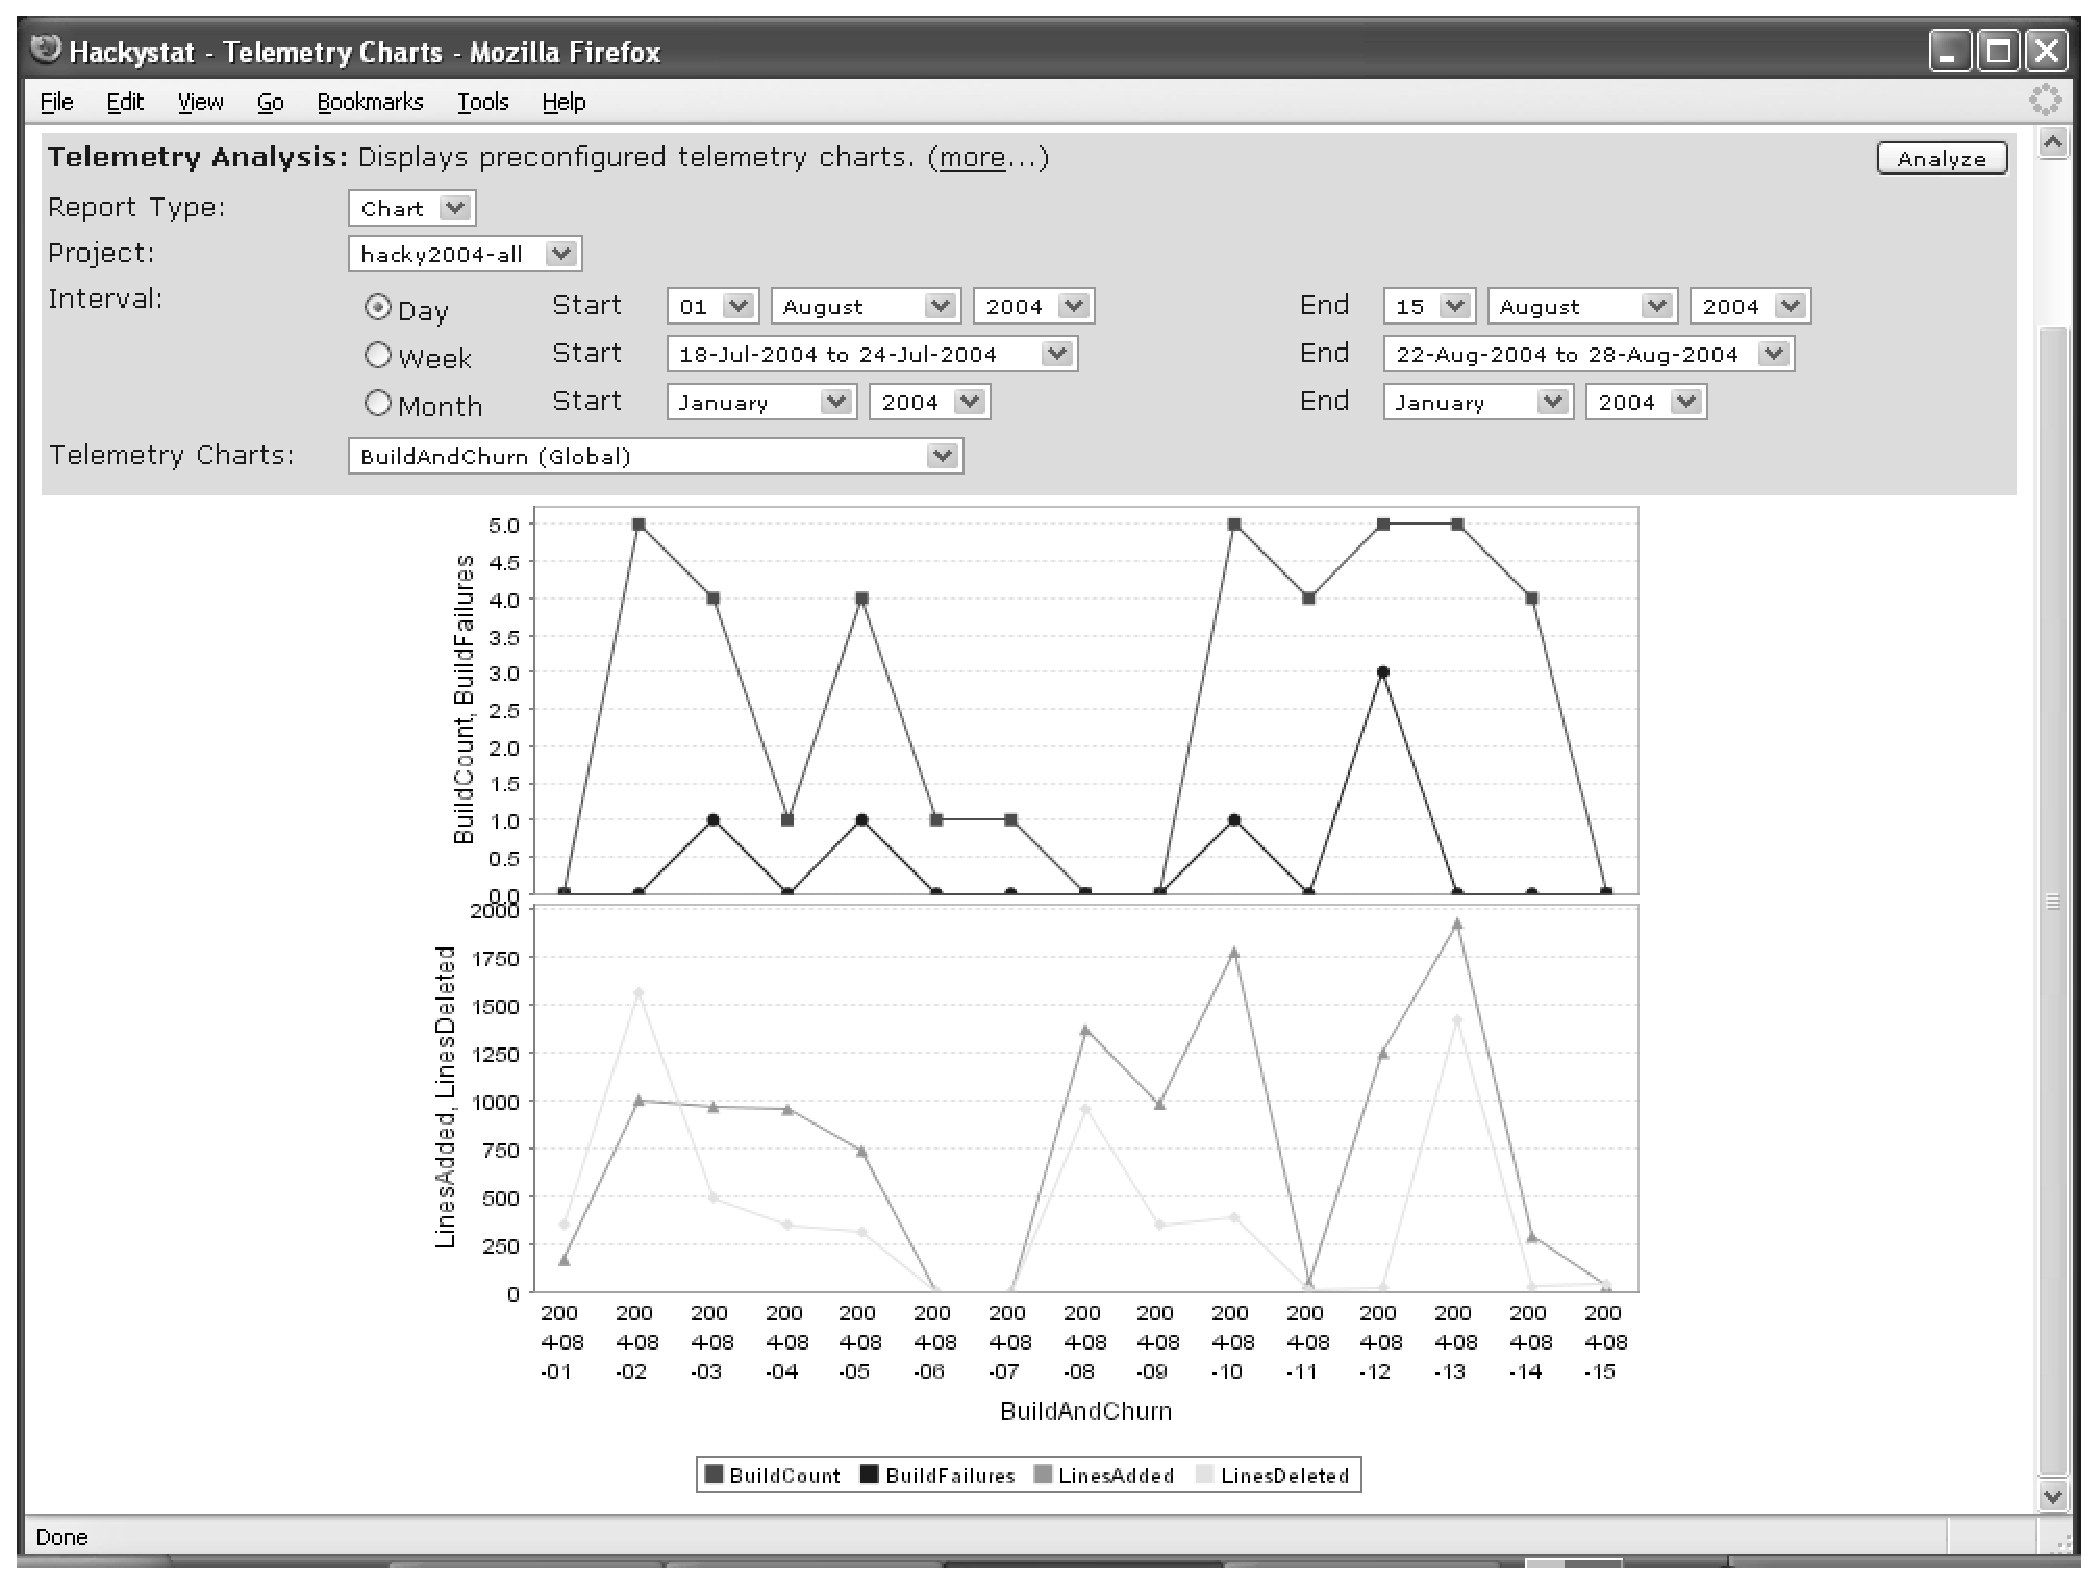
\includegraphics[width=0.75\textwidth]{BuildAndChurn.eps}
  \caption{A telemetry report that compares code churn (lines
  added and lines deleted) to build results (number of build attempts and
  number of failures.} 
  \label{fig:telemetryreport}
\end{figure*}

Figure \ref{fig:telemetryreport} shows an example telemetry report.  This
report illustrates the relationship between aggregate code churn (the lines
added and deleted from the CVS repository by all members of the project)
and aggregate build results (the number of build attempts and failures on a
given day via invocation of the Ant build tool).  Note that Telemetry
Reports are always defined without reference to a specific project or time
interval.  The specification of the project and time interval for
presentation in the report is specified when the report is generated, not
as part of its definition.  Thus, project members can now run this
telemetry report over differing sets of days, or else change the time scale
to Weeks for Months to see if different trends emerge from these
alternative perspectives.  In addition, once defined, members of other
projects on this server could use the BuildAndChurn telemetry report to see
if it adds decision-making value to their project management activities.

\Section{Telemetry in practice: managing integration build failure}

As a concrete example of software project telemetry in action, we are
currently using it to investigate and improve our own daily (integration)
build process.  Hackystat consists of approximately 65 KLOC, organized into
approximately 30 modules, with 5-10 active developers. The sources are
stored in the CVS configuration management system, allowing developers to
check out the latest version of the sources associated with any given
module, and commit their changes when finished.  Developers rarely compile,
build, and test against the entire code base, instead selecting a subset of
the modules relevent to their work.  An automated nightly build process
compiles, builds, and tests the latest committed code for all modules and
sends email if the build fails.  We can also invoke this integration build
manually.

At the end of 2004, we discovered that our integration build failure rate
was significant: for the 300 daily integration build attempts during that
year, the build failed on 88 of those days with a total of 95 distinct
build errors.  The impact on our productivity of this high failure rate is
substantial, since each integration build failure generally requires one or
more members of the team to stop concurrent development, diagnose the
problem, determine who is responsible for fixing it, and often wait until
the corrections have been committed before checking out or committing
additional code.

In order to reduce the rate of integration build failure in 2005, we needed
to understand more about how, when, and why the builds were failing in
2004. To do this, we embarked on a series of analyses involving several
Hackystat sensor data streams: Active Time, Commit, Build, and Churn.  This
revealed many useful insights about our build process.  First, we could
partition the 95 distinct build errors into six categories: Coding Style
Error (14), Compilation Error (25), Unit Test Error (40), Build Script
Error (8), Platform-related Error (3), and Unknown Error (5). Second, we
found substantial differences between experienced and new developers with
respect to integration build failures. For example, the least experienced
developer had the highest rate of integration build failure: an average of
one build failure per four hours of Active Time. In contrast, more
experienced developers averaged one build failure per 20 to 40 hours of
Active Time. Third, the two modules with the most dependencies to other
modules also had the two highest numbers of build failures, and together
accounted for almost 30\% of the failures. Fourth, we found that the 88
days with build failures had, on average, a statistically significant
greater number of distinct module commits than days without build failures.
Fifth, we found (somewhat unexpectedly) that there was no relationship
between build failure and the number of lines of code committed or the
amount of Active Time spent before the commit. In other words, whether you
worked five hours or five minutes before committing, and whether you
changed 5 lines of code or 500 didn't measurably change the odds of causing
a build failure.

These findings yield a number of hypotheses regarding ways to reducing
integration build failure, including increased support for new developers
such as pair programming, and refactoring of modules to reduce coupling and
the frequency of multi-module commits. The most provocative hypothesis,
however, is that 82\% of the 2004 integration failures could have been
prevented if the developers had run a full compile and test of the system
before committing their changes.  

The most simple, and most intrusive, process ``improvement'' would require
all developers to run a full compile and test of the system locally before
every commit. However, even though some commits without testing result in
an integration build failure, many other commits without testing do not.
Given that a full compile and test can take between 10-20 minutes depending
upon the machine, and that multiple developers often perform multiple
commits per day, the productivity cost of this process improvement could
actually exceed the benefits from reducing the current level of integration
build failures! Other ``generic'' changes, such as moving to continuous
integration, also tend to move the costs of build failure around without
necessarily reducing them.

Our current approach to managing integration build failure comes from
recognizing that the decision about whether to invest the time to perform a
full build and test before any particular commit is a complicated one,
involving developer familiarity with the system, the actual changes made to
the code, the commits being made concurrently by other developers, and so
forth.  To improve our productivity, we need to give developers the tools
and feedback necessary to better decide when a specific commit should be
proceeded by a full build and test.  To assess whether the feedback is
working, we can use Software Project Telemetry. 

Our analyses demonstrate that understanding the causes of success or
failure of any given integration build requires multiple forms of process
and product information, including the occurrence of local builds, the
success or failure of the integration build, the type of failure, the
modules that were committed, the developers responsible, the dependency
relationships between modules, and the Active Time associated with the work
prior to commits.  Unfortunately, we have not discovered any analytical
model that could automate the decision making process and tell a developer
before they commit whether full or partial testing is needed.  However,
using Software Project Telemetry, we can track the absolute level of
integration build failures over time, as well as the number due to any
particular cause, and even the number that could have been prevented by a
prior full build and test.  Using Hackystat's alert mechanism, we can
provide developers a detailed summary of the process and product state,
including the factors we have identified as relevent, whenever an
integration build failure occurs.  Our hypothesis is that, given
appropriate feedback, each developer will naturally learn over time to be
more sophisticated in deciding when to perform a full build and test.  New
developers might quickly learn to do it almost all of the time, while more
experienced developers might begin to recognize more complex indicators. 
One of our project goals for 2005 is to test this hypothesis, and measure
the results using integration build failure telemetry streams.


\Section {The Telemetry Control Center}

For a project of even moderate size and complexity, the number of possible
telemetry charts and reports quickly explodes.  For example, the
Hackystat development project is monitored by almost a dozen different sensor data
streams, across 30 modules, from 5-10 active developers.  Given that
each telemetry stream can be composed from one or more sensor data streams,
one or more project modules, and one or more developers, you can see the
problem: which of the literally thousands of possible charts should we be
monitoring? 

\begin{figure*}[ht]
  \centering
  \includegraphics[width=0.75\textwidth]{Wall.eps}

  \caption{The Telemetry Control Center, showing one ``scene'' consisting
  of nine telemetry reports. The associated TelemetryViewer software 
  controls the TCC by automatically cycling
  through a set of scenes at a predefined interval. This 
  telemetry viewer is configured to show a dozen separate
  scenes, each displayed for two minutes.  }
  \label{fig:telemetrycontrolcenter}
\end{figure*}

In our development group, we decided to address this problem by creating a
new interface to the telemetry data that would enable us to passively
monitor telemetry in a way that a standard web browser would not allow. We
call this interface the ``Telemetry Control Center'', as shown in Figure
\ref{fig:telemetrycontrolcenter}.  

The Telemetry Control Center consists of a standard PC with a multihead
video display card that is attached to nine 17'' LCD panels, mounted on the
wall in our laboratory.  We implemented a new client-side software system
called the TelemetryViewer, which periodically requests Telemetry Reports
from the Hackystat server, retrieves the resulting image file, and displays
them on screens.  The TelemetryViewer reads in an XML configuration file at
startup, which tells it which reports to retrieve, where to display them,
and how long to wait before retrieving the next set of reports. The default
behavior of the TelemetryViewer is to automatically and repeatedly cycle
through the set of telmetry ``scenes'' specified in the XML configuration
file.

The Telemetry Control Center frees us from the ``tyranny of the browser'',
by making a sequence of telemetry report sets continuously available
without any action on the part of developers. It also enables us to more
easily look for relationships between telemetry streams, since the system
can display nine telemetry reports simultaneously.  Finally, it provides a
new kind of passive awareness about the state of the project to all
developers; rather than having to decide to generate a report or wait for a
weekly project update meeting, developers can simply glance at the
Telemetry Control Center whenever they are passing though the lab to get a
perspective on the state of development. Of course, individuals can still get all of the Telemetry Control Center reports 
on their local workstations if they so desire, although without the simultaneous display.

\Section{Lessons Learned}

Our first lesson learned is that software project telemetry can provide
useful support for project management decision making. In addition to our
work on integration build failure, telemetry data has also revealed to us a
recent, subtle slide in testing coverage over the past six months that has
co-occurred with two episodes of significant refactoring (and resulting
code churn).  As a result, we are allocating additional effort to software
review with a focus on assessing the test quality of new modules.  We hope
that this project management decision will lead to a reversal of the
declining coverage trend.

Hackystat provides an open source reference framework for Software Project
Telemetry, but Hackystat is not the only technology available.  Commercial
measurement tools can also provide infrastructure support, or your
organization could decide to develop technology in-house. The key issue is
to preserve the essential properties of software project telemetry.

We have learned that having an automated daily build mechanism adds
significant value to software project telemetry. It both provides a
convenient hook into which you can add sensors to reliably obtain daily
information about product measures, but also provides a kind of heart beat
for the development project that makes all the metrics more comparable,
accessable, and current.

As with any measurement approach, social issues must be taken into
account. It is possible to misinterpret and misuse software project
telemetry data. For example, telemetry data is intrinsically incomplete
with respect to measuring ``effort''.  Hackystat implements a measure
called Active Time, which is the time developers and managers spend editing
files related to a given project in tools such as Eclipse, Word, or
Excel. However, many legitimate and productive activities, including
meetings, email, and hallway conversations are outside the scope of
telemetry-based measurement. Telemetry cannot measure ``effort'' in its
broadest sense, and a small value of Active Time by a project member does
not necessarily imply that they are not contributing a great deal of
productive effort to the project.  Indeed, some organizations may decide
not to collect measures such as Active Time, simply because it is
susceptible to misinterpretation and/or abuse.  Robert Austin provides
an excellent analysis of these and other forms of ``measurement dysfunction'' \cite{Austin96}. 


The adoption of a software project telemetry approach to measurement and
decision making tends to exert a kind of gravitational force toward
increased use of tools for managing process and products. For example, a
small development team might begin by informally managing tasks and defects
using email or index cards.  As they start to adopt telemetry-based
decision making, they will inevitably want to relate development process
and product characteristics to open tasks, defect severity levels, and so
forth, but not be able to do so unless they move to an issue management
tool such as Bugzilla or Jira that enables sensor-based measurement.


\Section{Future directions}

Does software project telemetry provide a silver bullet that solves all of
the problems associated with metrics-based software project management and
decision making?  Of course not.  While software project telemetry does
address certain problems inherent in traditional measurement, and provide a
new approach to more local, in-process decision-making, it provides its own
set of issues that must be addressed by future research and practice.

First, the decision-making value of telemetry data is only as good as the
quality and diversity of data that can be obtained by sensors. Clearly,
there is some threshold for sensor data, beneath which the decision-making
value of software project telemetry is compromised. But what is this
threshold, and how does it vary with the kinds of decision-making required
by the development group?  What set of sensors and sensor data types are
best suited to what project development contexts?

Second, what are the intrinsic limitations to telemetry-based data?
A good way to investigate this question involves qualitative, ethnographic
research, in which a researcher trained in these methods observes a
software development group to learn what kinds of information relevant to
project management decision-making occur outside of the realm of telemetry
data. 

Third, while manual investigation of telemetry streams and their
relationship to each other is certainly an important and necessary first
step, the sheer number of possible relationships and interactions means
that only a small percentage of them can be inspected and monitored
manually on an ongoing basis.  An intriguing future direction is to explore
the use of data mining and clustering algorithms to see if they can reveal
relationships in the telemetry data that might not be discovered through
manual exploration. 

Fourth, what are the costs associated with initial setup of Software
Project Telemetry using a system like Hackystat? Unfortunately, we cannot
use Hackystat to measure the effort involved with installation of
Hackystat.  Furthermore, some organizations will require development of new
sensors or analyses not available in the standard distribution.  Better
understanding of these costs will aid adoption of this technology and
method.



\Section{Sidebar: Sensors and Sensor Data Types}
\label{sec:Sidebar:Sensors}

Hackystat provides an extensible architecture with respect to both
``sensors'', or the software plugins associated with development tools, and
``sensor data types'', which describe the structure of a given type of raw
metric data.  This mapping is not one-to-one: for example, the Eclipse
sensor can send Activity, FileMetric, and Review sensor data types, and the
FileMetric sensor data type can be collected by both IDE and Size metric
sensors.   The following lists describe the range of currently available
sensors and sensor data types; each organization can decide whether or not
to enable these facilities, or whether to implement their own custom
extensions to better facilitate their own needs.

Hackystat sensors are currently implemented for the following tools:
\begin{itemize}
\item {\em Interactive development environments}, including Eclipse, 
Emacs, JBuilder, Vim, and Visual Studio;
\item {\em Office productivity applications}, including Excel, Word,
Powerpoint, and Frontpage;
\item {\em Build tools}, including Ant and the Unix command line;
\item {\em Size measurement tools}, including CCCC and LOCC;
\item {\em Testing tools}, including JUnit and JBlanket;
\item {\em Configuration management}, including CVS and Harvest;
\item {\em Defect tracking tools}, including Jira;
\end{itemize}

Hackystat sensor data types include:
\begin{itemize}
\item {\em Activity}, which represents data concerning the active time spent
by developers in their IDE;
\item {\em BufferTransitions}, which represents the sequence of files visited
by developers;
\item {\em Review}, which represents data on review issues generated during
code or design inspections;
\item {\em FileMetric}, which represents size information about files;
\item {\em Build}, which represents data about the occurrence and
outcome of software builds.
\item {\em Perf}, which represents data about the occurrence and outcome of
performance analysis activities such as load testing;
\item {\em CLI}, which represents data about the occurrence of command line
invocations;
\item {\em UnitTest}, which represents data about the occurrence and
outcome of unit test invocations;
\item {\em Coverage}, which represents data about the coverage obtained by
unit testing activities;
\item {\em Commit}, which represents data about configuration management
commit events by developers;
\item {\em Defect}, which represents information about the posting of
defect reports to defect tracking tools by developers or users
\end{itemize}

Hackystat is an open source system that is freely available for
download and use. We encourage interested theorists and practitioners to
visit the developer services website at http://www.hackystat.org,
where access to source, binaries, and documentation is available. To try out
Hackystat, we also maintain a public server at http://hackystat.ics.hawaii.edu.


\Section{Acknowlegements}

We gratefully acknowledge support for Project Hackystat by the NSF and NASA
as part of their joint program on Highly Dependable Systems, by Sun
Microsystems as part of the DARPA High Productivity Computing Systems
program, and by IBM as part of the Eclipse Innovation Grant program.

\bibliographystyle{/export/home/csdl/tex/icse2003/latex8}
\bibliography{/export/home/csdl/techreports/04-11/04-11,/export/home/csdl/bib/csdl-trs,/export/home/csdl/bib/hackystat,/export/home/csdl/bib/psp}
\end{document}
 










